\documentclass[class=book, crop=false, oneside]{standalone}
\usepackage[subpreambles=true]{standalone}

\usepackage{../../style}

\graphicspath{{./assets/images/}}
\newmintinline{asm}{}

% arara: pdflatex: { synctex: yes, shell: yes }
% arara: latexmk: { clean: partial }
\begin{document}
\chapter{Central Processing Unit}

In questo capitolo andremo ad analizzare come il nostro processore elabora ed esegue le istruzioni che gli arrivano dai programmi Assembly; in particolare ci baseremo ancora su MIPS, in quanto super regolare e particolarmente utile a scopo didattico.\\

\section{Introduzione}
Per come è stato progettato MIPS, le istruzioni presentano dei tratti comuni;in particolare le prime due fasi del ciclo della CPU (vedi~\ref{subsec:cpu}), ossia il prelievo dell'istruzione e la lettura dei valori dei registri operandi sono comuni a ogni istruzione.\\
Noi in particolare, dopo aver spiegato i vari elementi che concorrono a far funzionare tutta la baracca, andremo ad analizzare le istruzioni aritmetico-logiche, quelle di accesso alla memoria e quelle di salti, dal momento che tutte le altre si implementano con tecniche simili.

\section{Arithmetic-Logic Unit}
A eccezione di \mintinline{asm}{j}, tutte le istruzioni MIPS fanno uso di \emph{arithmetic-logic unit} (ALU per gli amici), una rete logica combinatoria abbastanza complessa preposta all'esecuzione di tutti calcoli di cui abbiamo bisogno; sostanzialmente, è un’unione di blocchi fondamentali che fanno operazioni su singoli bit.\\
Al di là delle operazioni puramente aritmetiche (per le quali lo scopo di ALU è ovvio), viene usato nelle operazioni di accesso alla memoria (\mintinline{asm}{sw} e \mintinline{asm}{lw}) per il calcolo degli indirizzi e dalle operazioni di salto condizionato per effettuare i confronti; successivamente, ognuna di queste tre categorie differisce. \\

\section{Il datapath}
Il \emph{datapath} è quella parte del processore attraverso cui passano le istruzioni; è letteralmente un percorso da seguire ogniqualvolta si voglia esegire una qualsiasi istruzione.

\subsection{Struttura del datapath}
\begin{figure}[H]
	\centering
	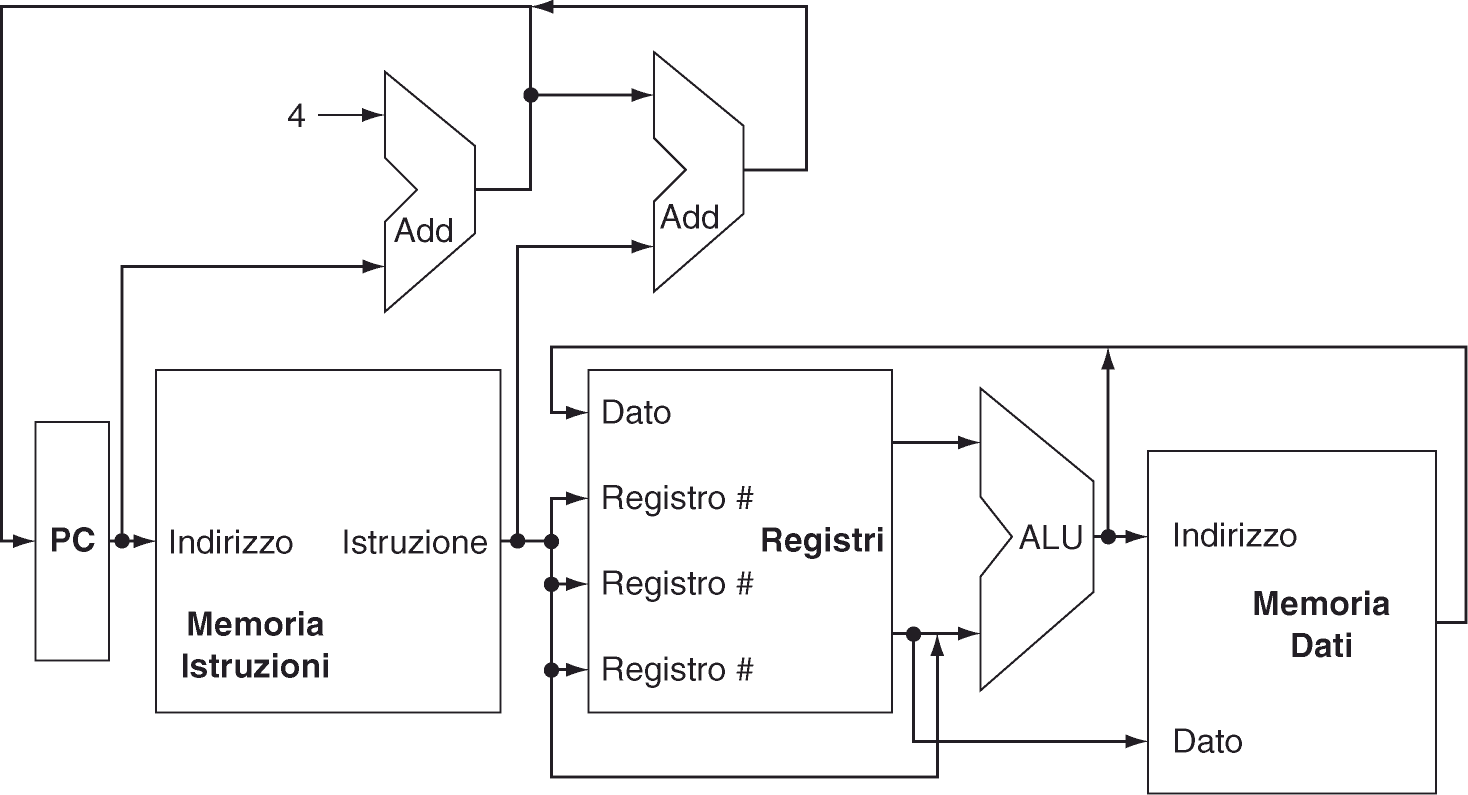
\includegraphics[width=0.9\textwidth,keepaspectratio]{datap_1}
	\caption{Schema base del datapath}
\end{figure}
Il datapath si compone essenzialmente di 5 fasi:
\begin{enumerate}
  \item assumendo che il programma sia già stato caricato in memoria (secondo le modalità viste nel capitolo~\ref{ch:tool}), in questa fase viene prelevata l'istruzione da eseguire e viene spacchettata nei vari campi;
  \item i registri interessati all'esecuzione vengono caricati nel \emph{banco dei registri}; se l'istruzione è di tipo R, gli indirizzi dei registri sono contenuti nel corpo dell'istruzione;
  \item a questo punto la ALU esegue i calcoli opportuni, ottenendo il valore (o l’indirizzo) desiderato;
  \item i risultati ALU vengono utilizzati per salvare (o prelevare) in memoria dati un dato, o per emorizzare un registro;
  \item si incrementa il program counter per mezzo di una ALU dedicata (di fatto, un addizionatore), e una successiva ALU calcola l’indirizzo verso cui mi dovrò spostare in caso di salti incondizionati;
\end{enumerate}

\subsection{Il ruolo del multiplexer}
La  figura però è incompleta; manca qualcosa che dica ai blocchi cosa fare in caso di punti di decisione (momenti in cui i segnali arrivano da due diverse sorgenti e bisogna sceglierne una), come ad esempio l'incremento del program counter: normalmente, il suo valore proviene dall'addizionatore (e punta quindi alla word successiva a quella appena letta), ma in caso di salto l'indirizzo viene calcolato dallo spiazzamento contenuto nell'istruzione.\\
Altro esempio: a seconda della tipologia di istruzione il secondo operando della ALU potrà provenire o dal banco dei registri (per le istruzioni R) o dal codice dell'istruzione stessa (per le istruzioni I).\\
Ed è qui che ci viene in soccorso il \emph{multiplexer} che, come già detto in~\ref{subsec:multi}, è un circuito combinatorio che prende in input due segnati e decide quale di essi debba andare in output sulla base di un terzo segnale di controllo (un po' come un vigile che decide quale macchina far passare).
\begin{figure}[H]
	\centering
	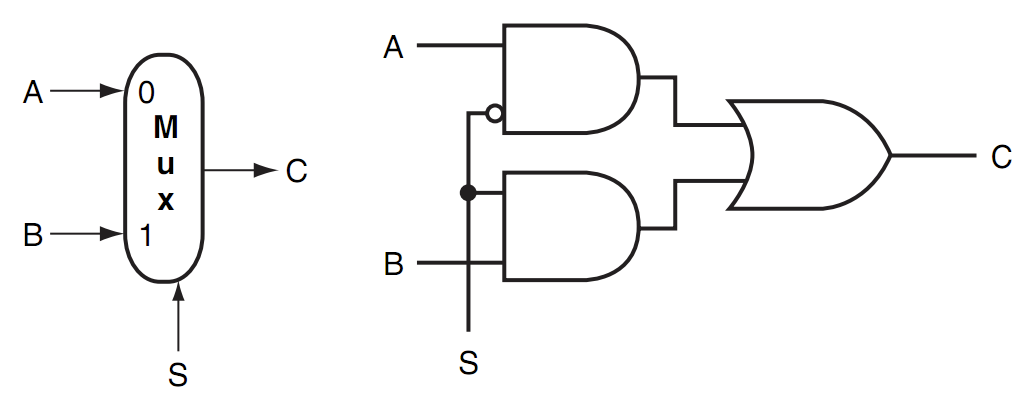
\includegraphics[width=0.9\textwidth,keepaspectratio]{multi}
	\caption{Schema di un multiplexer}
\end{figure}
\paragraph{Altri elementi}
Oltre ai multiplexer, ci sono altri elementi che concorrono alla soluzione dei punti di decisione. Ad esempio le ALU ha diversi ingressi per decidere quale operazione effettuare e il banco dei registri ha delle porte per decidere se scrivere o meno un registro, e la memoria dati ha degli espedienti per decidere se effettuare lettura o scrittura.\\
E chi stabilisce queste cose, oltre a settare il segnale del selettore dei vari multiplexer?  È presto detto, l’unità di controllo!\\

\section{La control unit}
La \emph{control unit} funge da vero e proprio "direttore d'orchestra" per il processore, stabilendo il valore \(S\) dei vari multiplexer.
\begin{figure}[H]
	\centering
	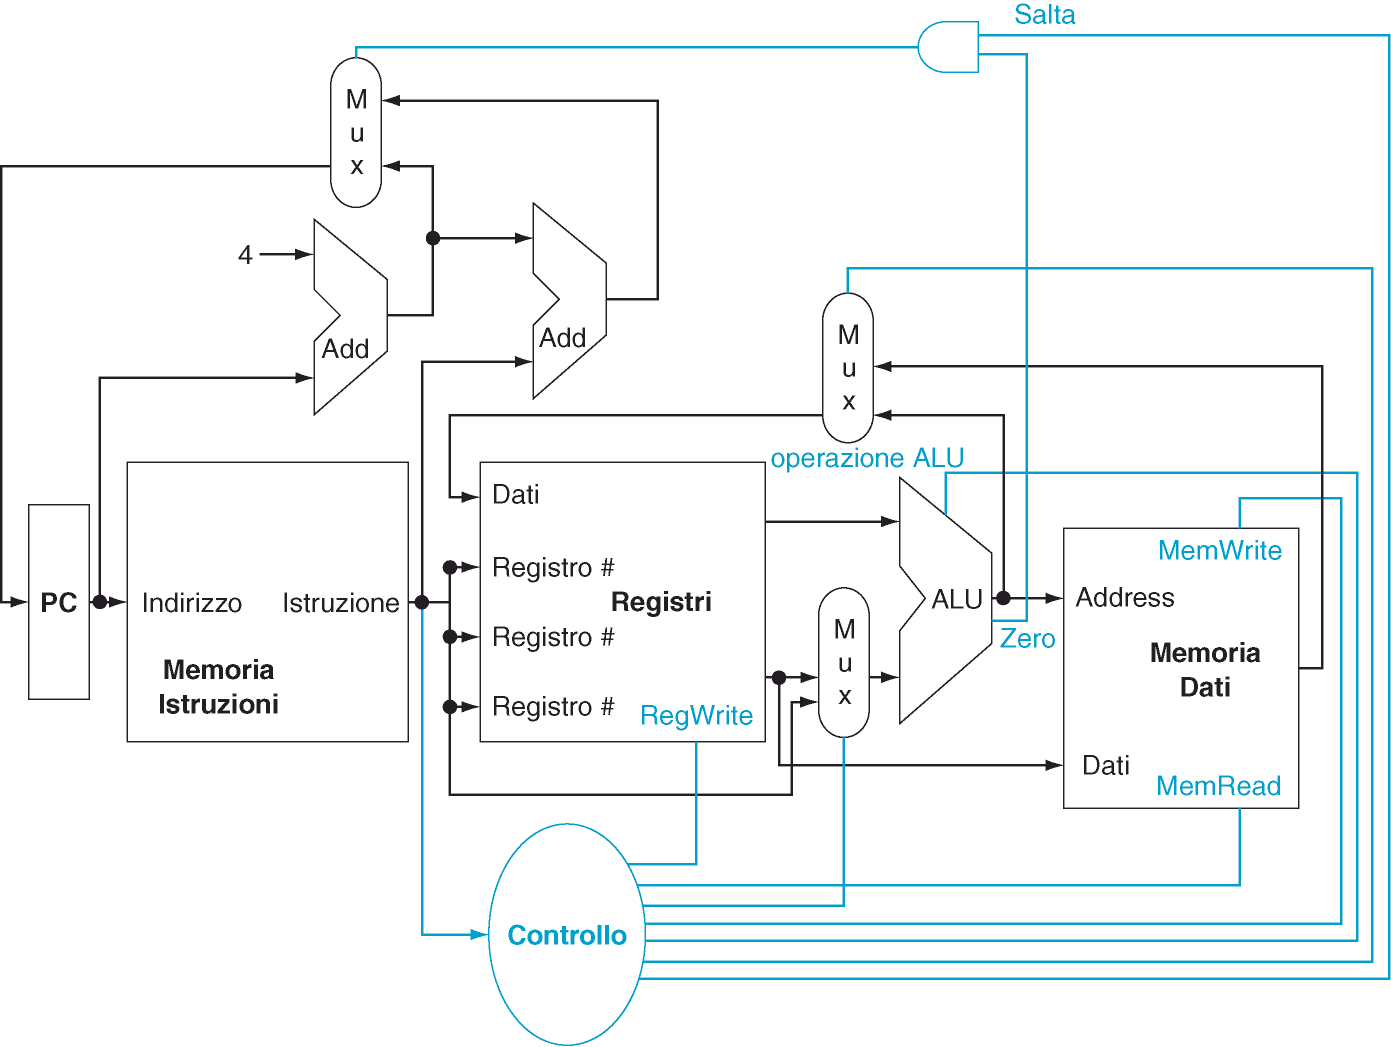
\includegraphics[width=0.9\textwidth,keepaspectratio]{datap_2}
	\caption{Schema di datapath e control unit}
\end{figure}
C’è un MUX prima del PC che prende il primo blocco add del pc come primo operando e il secodno come, be’, secondo; il selettore è SALTA, che decide se stiamo facendo (dritto o storto? Che cazzo fa?)\\

Ok allora c’è il blocco che vede se stiamo facendo un operazione di salto che va dentro a un and, e il risultato dell’and va come selettore\\

Ce n’è uno anche per il discorso di prendere l’indirizzo di destinazione e per scegliere se andare a leggere o scrivere in memoria\\

Stessa cosa per quanto riguarda la scelta del caricamento di un registro o una costante come secondo operando, sempre gestita da un MUX direttamente gestito dall’unità di controllo\\

Uno va dentro alla ALU, che è un bus di più bit per scegliere il tipo di operazione svolta dall’unità
Regwrite dice di scrivere il registro (decisamente da approfondire)\\

LE ARCHITETTURE CISC SONO MOLTO PIÙ COMPLESSE DI COSÌ\\

A questo punto abbiamo moltissimi segnali che viaggiano nel processore, si manifesta la necessità di sincronizzarli, ed è a questo che serve il CLOCK (assumiamo che tutte le istruzioni vengano eseguite con un singolo colpo di clock lungo abbastanza\\

Reti sequenziali hanno un valore DI STATO, e hanno due ingressi: valori di stato (registri in ingresso) e un clock per sincronizzare le transizioni di stato\\

Il flip-flop d-latch è l’elemento base per memorizzare un bit, e registri sono vettori di flip flop\\

TEMPORIZZAZIONE: quando faccio una lettura, sono sicuro che quello che sto leggendo è ciò che e stato scritto al ciclo precedente, e che quindi la sequenza delle cose è quella\\

Il tempo T di clock deve essere tale da dare tempo ai dati di attraversare le reti ed è fondamentale perché altrimenti l’output prodotto sarebbe una merda, perché non sapremmo quando leggere il dato e che dato stiamo leggendo; grazie al tempo, possiamo avere indicazioni molto precise\\

Andando a rivedere il datapath, abbiamo memoria istruzioni, pc e l’addizionatore\\

Ogni ciclo di clock viene effettuato un fetch, viene resa disponibile l’istruzione e viene incrementato il program counter\\

Andiamoa  vedere l’esecuzione di un’istruzione R: mi servono anche il banco dei registri (con 3 bus da 5 bit ciascuno) e un’ALU (con settare un bit per l’and del pc se il risultato è 0), se ho operazione aritmetica. Inoltre ho il controllo RegWrite per vedere se sto leggendo o scriveno sul banco registri\\

Per le istruzioni di load e store bisogna calcolare un indirizzo di memoria dato da indirizzo e offset, quindi continua a servirci la ALU; abbiamo inoltre bisogno di un segnale di controllo per vedere se stiamo scrivendo o meno\\

Abbiamo bisogno anche di un circuito di memoria dati per l’estensione del segno, per estendere da 16 a 32 bit
(Salto condizionale)


\end{document}
